%start preamble
\documentclass[paper=a4,fontsize=11pt]{scrartcl}%kind of doc, font size, paper size

\usepackage{fontspec}
\defaultfontfeatures{Ligatures=TeX}
%\setsansfont{Liberation Sans}
\usepackage{polyglossia}	
\setdefaultlanguage[spelling=new, babelshorthands=true]{german}
\usepackage{csquotes}
		
\usepackage{amsmath}%get math done
\usepackage{amsthm}%get theorems and proofs done
\usepackage{graphicx}%get pictures & graphics done
\graphicspath{{pictures/}}%folder to stash all kind of pictures etc
\usepackage[hyphens]{url}
\usepackage{amssymb}%symbolics for math
\usepackage{amsfonts}%extra fonts
\usepackage []{natbib}%citation style
\usepackage{caption}%captions under everything
\usepackage{listings}
\usepackage[titletoc]{appendix}
\numberwithin{equation}{section} 
\usepackage[printonlyused,withpage]{acronym}%how to handle acronyms
\usepackage{float}%for garphics and how to let them floating around in the doc
\usepackage{cclicenses}%license!
\usepackage{xcolor}%nicer colors, here used for links
\usepackage{wrapfig}%making graphics floated by text and not done by minipage
\usepackage{dsfont}
\usepackage{stmaryrd}
\usepackage{geometry}
\usepackage{fancyhdr}
\usepackage{menukeys}
\usepackage{enumitem}

\pagestyle{fancy}
\lhead{Netzwerke Übung\\SoSe2020}
\rhead{FB 4 -- Angewandte Informatik\\ HTW-Berlin}
\lfoot{Grundlagen Linux \& Shell}
\cfoot{}
\fancyfoot[R]{\thepage}
\renewcommand{\headrulewidth}{0.4pt}
\renewcommand{\footrulewidth}{0.4pt}

\lstdefinestyle{Bash}{
  language=bash,
  showstringspaces=false,
  basicstyle=\small\sffamily,
  numbers=left,
  numberstyle=\tiny,
  numbersep=5pt,
  frame=trlb,
  columns=fullflexible,
  backgroundcolor=\color{gray!20},
  linewidth=0.9\linewidth,
  %xleftmargin=0.5\linewidth
}

%%here begins the actual document%%
\newcommand{\horrule}[1]{\rule{\linewidth}{#1}} % Create horizontal rule command with 1 argument of height

\begin{document}
\center
\Large{Fakultative Aufgaben -- Shell Grundlagen}
\begin{center}\Large{\textbf{Shell}}\end{center}\vskip0.25in
%\setlist[enumerate, 1]{itemsep=\baselineskip}
\begin{enumerate}
	\item Mit welchem Kommando können Sie ...
   \begin{enumerate}[label=(\alph*)]
   \item Handbuchseiten (Man Pages) öffnen
   \item das aktuelle Verzeichnis in der Shell ausgeben?
   \item den Inhalt eines Verzeichnisses in der Shell ausgeben?
   \item eine leere Datei erzeugen?
   \item versuchen den Inhalt einer Datei zu bestimmen?
   \item den Inhalt verschiedener Dateien verknüpfen oder den Inhalt einer Datei ausgeben?
   \item Zeilen vom Ende einer Datei in der Shell ausgeben?
   \item Zeilen vom Anfang einer Datei in der Shell ausgeben?
   \item ein leeres Verzeichnis löschen?
   \item eine Zeichenkette in der Shell ausgeben?
   \item Das Password eines Benutzers ändern?
   \item das System neu starten?
   \item das System ausschalten
   \item einen neuen Benutzer erstellen?
   \item einen Benutzer löschen?
   \item einen Benutzer ändern?
   \item eine Liste der laufenden Prozesse in der Shell ausgeben?
   \item einen Prozess beenden?
   \item eine Gruppe von Prozessen beenden?
   \item eine Liste der existierenden Prozesse als Baumstruktur in der Shell ausgeben?
	\end{enumerate}
\end{enumerate}
   \begin{center}\Large{\textbf{CLI-Editoren}}\end{center}\vskip0.25in
   \begin{enumerate}
   		\item Jedes Linux/ Unix verfügt über den Editor \emph{vi}, bearbeiten Sie folgendes Tutorial:\\
  \url{https://www.tutorialspoint.com/unix/unix-vi-editor.htm}\\
  Alternativ können Sie auch mit dem \emph{vim} arbeiten, dieser ist eine Erweiterung des \emph{vi} und etwas einfacher zu bedienen.
  		\item Alternativ steht auch der Editor \emph{emacs} zur Verfügung. Entsprechend können Sie folgendes Tutorial durcharbeiten:\\
  		\url{https://www.gnu.org/software/emacs/tour/}
\end{enumerate}

\begin{center}\Large{\textbf{Umgebungsvariablen, Links \& Default-Shell}}\end{center}\vskip0.25in
%\setlist[enumerate, 1]{itemsep=\baselineskip}
\begin{enumerate}
\item Was sind Umgebungsvariablen, wozu werden diese gebraucht?
\item Ändern Sie die PS1-Variablen ihrer Shell derart um, dass Ihre Shell-Umgebung den Nutzernamen @ Hostnamen gefolgt von der Urzeit und in einer neuen Zeile den aktueller Pfad gefolgt von einem Leerzeichen und dem \$-Zeichen. Womit ihre Shell etwa wie folgt aussehen sollte:
\begin{figure}[H]
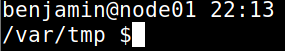
\includegraphics[scale=0.6]{ps1}
\end{figure}
\item Worin besteht der Unterschied zwischen Hard- und Soft-Links?
\item Als Standard-Shell ist auf den Laborrechnern als BASH voreingestellt, wie könnte man dies ändern? Auf dem Raspberry Pi ist momentan die Bourne-Again-Shell (bassh) eingestellt, als Alternativen stehen die Bourne-Shell (BASH) und die Z-Shell (ZSH) (mitsamt OhMyZSH) zur Verfügung. Es gibt noch viele weitere Kommandozeileninterpreter. Recherchieren Sie, was man unter dem Begriff Kommandozeileninterpreter versteht. \footnote{Suchen nach dem Unterschied zwischen interpretierten und kompilierten Sprachen!}.\\
Versuchen Sie ganz wesentliche Unterschiede zwischen Bourne-Shell und BASH/ZSH herauszufinden.
\item Auf den Laborrechnern befinden sich alle eben genannten Shells, Sie können ihre Default-Shell mithilfe des Befehls\\
    \begin{lstlisting}[style=Bash, language=Bash]
chsh [-s /path/to/shell] [s05XXXXX]
		\end{lstlisting}
		ändern. 
\end{enumerate}
\begin{center}\Large{\textbf{Advanced Tools -- grep, awk \& sed}}\end{center}\vskip0.25in
Jede Shell unter Unix hat einige sehr mächtige Tools (sed \& awk sind eigentlich richtige Programmiersprachen!). Diese Werkzeuge sind wahre Allrounder in Sachen Textverarbeitung.
\begin{enumerate}
	\item global regular expression print (grep) ist eine Werkzeugsammlung, mit deren Hilfe Texte und Datein durchsucht werden kann. Durch den Einsatz von Regulären Ausdrücken (regualar expressions -- kurz regex) kann dies äußert effizient sein. Bearbeiten Sie folgendes Tutorial: \url{https://www.uccs.edu/~ahitchco/grep/} oder\\
	\url{https://www.thegeekstuff.com/2009/03/15-practical-unix-grep-command-examples/}
	\item awk (Aho Weinberger Kernighan) ist eine schon etwas ältere Programmiersprache von Alfred Aho (Dragon Book -- Compilerbau), Peter J. Weinberger und Brian Kernighan (Unix, C).\\
	Bearbeiten Sie folgendes Tutorial: \url{https://www.tutorialspoint.com/awk/index.htm}
	\item sed (stream editor) ist eine Programmiersprache und Unix-Tool von Lee E. McMahon (comm, qsort, grep) zur effizienten Textbearbeitung.\\
	Bearbeiten Sie folgendes Tutorial: \url{https://www.tutorialspoint.com/sed/index.htm}
	\item Wenn Sie weiteren Übungsbedarf haben kann ich Folgende Seite empfehlen:\\
	\url{https://www.hackerrank.com/domains/shell/bash}\\
	Hier finden Sie eine schöne Sammlung exemplarischer Aufgaben, die mit den oben genannten Tools gelöst werden kann. Darüber hinaus bietet hackerrank eine Fülle an Übungsaufgaben in den Bereichen Algorithmen, Datenstrukturen, Programmiersprachen etc.
\end{enumerate} 
\end{document}